\documentclass[11pt,border=5pt]{standalone}
\usepackage{fontspec}
\setmainfont{cmunrm.otf}[BoldFont=cmunbx.otf,ItalicFont=cmunti.otf,BoldItalicFont=cmunbi.otf]
\usepackage{amsmath}
\usepackage{unicode-math}
\setmathfont{NewCMMath-Regular.otf}
\usepackage{tikz}
\usetikzlibrary{arrows.meta,patterns,angles,quotes}
\begin{document}
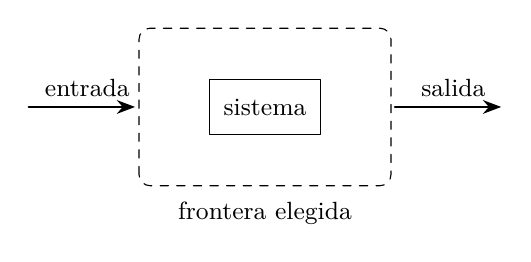
\begin{tikzpicture}[>=Stealth,font=\small,line cap=round,line join=round]
\draw[dashed,rounded corners] (-1.6,-1) rectangle (1.6,1);
\draw[fill=white] (-0.7,-0.35) rectangle (0.7,0.35);
\node at (0,0) {sistema};
\node at (0,-1.35) {frontera elegida};
\draw[->,thick] (-3,0) -- (-1.65,0) node[pos=0.55,above] {entrada};
\draw[->,thick] (1.65,0) -- (3,0) node[pos=0.55,above] {salida};

\end{tikzpicture}
\end{document}
